\documentclass{article}

% if you need to pass options to natbib, use, e.g.:
%     \PassOptionsToPackage{numbers, compress}{natbib}
% before loading neurips_2022

% ready for submission
\usepackage[preprint]{neurips_2022}

% to compile a preprint version, e.g., for submission to arXiv, add add the
% [preprint] option:
%     \usepackage[preprint]{neurips_2020}

% to compile a camera-ready version, add the [final] option, e.g.:
%     \usepackage[final]{neurips_2020}

% to avoid loading the natbib package, add option nonatbib:
%\usepackage[nonatbib]{neurips_2020}
\usepackage[utf8]{inputenc} % allow utf-8 input
\usepackage[T1]{fontenc}    % use 8-bit T1 fonts
\usepackage{hyperref}       % hyperlinks
\usepackage{url}            % simple URL typesetting
\usepackage{booktabs}       % professional-quality tables
\usepackage{amsfonts}       % blackboard math symbols
\usepackage{nicefrac}       % compact symbols for 1/2, etc.
\usepackage{microtype}      % microtypography


% Graphics and color
\usepackage{graphicx}
\usepackage{xcolor}

% Figures
\usepackage{subcaption}

% References and Bibliography
\usepackage[numbered]{bookmark} % Fixes false PDF table of contents
\usepackage{natbib}
\setcitestyle{numbers,sort&compress,square,comma}
\usepackage{bibentry}
\nobibliography*
\usepackage{url}
\usepackage{hyperref}
\hypersetup{
  colorlinks,
  linkcolor={black},
  citecolor={blue!50!black},
  urlcolor={blue!50!black}
}
\usepackage{cleveref}


\title{Can Plant-based Diets Help Solve Climate Change?}


\author{%
  Hanna Dettki\thanks{Equal contribution.}\hspace{4em} Davide Mornatta$^{*}$  \\[0.5em]
  Department of Computer Science\\
  University of Tübingen\\
  \texttt{\{hanna.dettki, davide.mornatta\}@student.uni-tuebingen.de}
  % \AND
  % Coauthor \\
  % Affiliation \\
  % Address \\
  % \texttt{email} \\
  % \And
  % Coauthor \\
  % Affiliation \\
  % Address \\
  % \texttt{email} \\
  % \And
  % Coauthor \\
  % Affiliation \\
  % Address \\
  % \texttt{email} \\
}

\begin{document}

\maketitle

\begin{abstract}
  Food is responsible for one quarter of the world's greenhouse gas (GHG) emissions \cite{Poore2018}, one of the main drivers of climate change. Providing a nutritious diet for the ever-growing world population while combatting global warming at the same time therefore poses a major challenge. This yields the question whether there are diets that are both sustainable for the climate and meet  nutritional requirements. In this study, we investigate if plant-based diets  emit significantly less GHG than animal based-products. We found  that plant-based food groups have significant lower GHG-emissions not only with respect to total emissions but also when controlling for nutritional value. For people wanting to  modify their lifestyle towards a more sustainable one both for the planet and their health, as growing body of research suggests \cite{WHO2021}, an easy rule to guide their daily food-decisions derived from this study would be to eat more plant-based.
\end{abstract}

\section{Introduction}

Climate change presents a major global threat. In order to avoid a climate disaster, radical change is needed. This concerns everything, from policies on a global and national level, to choices taken by the individual on a daily basis \cite{IPCC}. 
However, individuals motivated and willing to solve climate change by pursueing a sustainable life are faced with many obstacles to do so effortlessly. According to the UN, food, energy and water are the culprits for an unsustainable world, in particular in light of rapid population growth \cite{Ritchie2020}.
 Importantly, food systems are responsible for a third of global anthropogenic greenhouse gas emissions \cite{Crippa2021}. At the same time, food choices are to a large extent up to the individual.  However,  the emission cost of different food options are  typically not accessible, which is why individuals are  not easily able to adhere to  a climate-friendly diet. This shows that a significant lever contributing to solving climate change is not pulled.
\paragraph*{Research Question}
Therefore, we investigate the environmental impact of the most common food categories, which is a first step towards  providing more information in the jungle of food choices that everybody is presented with. In particular, we hypothesize that  plant-based diets  have a significantly smaller CO$_2$-footprint than  diets including animal-derived products. %in the typical Western diet.

\section{Data}
\label{data}
\paragraph{Data generating process} \label{dataGen}
The data used in this analysis  is the largest meta-analysis of food systems to date and was published in the journal \textit{Science} by \citet{Poore2018}.
570 studies met the eleven criteria\footnote{Such as  methodologies used were standardized, e.g., that all stages of the supply chain were considered.} \citet{Poore2018}  were applying to the initially  1530 studies.
The final dataset covers approximately 38,700 farms across 119 countries and spans a total of 40 food products, which represent approximately 90\% of global protein and calorie intake. The breadth of this analysis ensures that results are only minimally biased towards any geographic region,  any particular faming method or income level.
\paragraph*{Greenhouse gases (GHG) and how they are quantified}
Since there are many different greenhouse gases (GHG), researchers commonly aggregate them into a measurement that is easy to use for comparisons. 
\citet{Poore2018} use the metric 
``carbon dioxide-equivalents (CO$_{2}$eq)'', which is the most common measurement and is for instance  also used as a target-setting metric in official reportings like the Paris Agreement. CO$_{2}$eq express the ``global warming potential'' by aggregating the impact of all GHG into a single metric  and  aims to represent the amount of warming that each specific gas generates relative to CO$_2$. The ``global warming potential over a $100$-year timescale (GWP$_{100}$)'' expresses the mid- to longterm period for climate-policies. To calculate the CO$_{2}$eq-value, the amount of each GHG needs to factorized by its GWP$_{100}$-value. For example, the Intergovernmental Panel on Climate Change (IPCC) sets the GWP$_{100}$-value of the GHG  methane to $28$, which is based on the rationale that methane's global warming impact over a period of 100 years, will be $28$ times higher than that of one kilogram of CO$_2$ \cite{IPCC}.
%\paragraph{Stages of supply chain}
%Note: only if included in analysis
% Land use change; 
% On-farm impacts in crop or livestock production (including the manufacturing of inputs such as fertilizers, or emissions from manure);
% Animal feed production;
% Food processing: the conversion of raw ingredients into sold products, such as the processing of cereals into bread;
% Transport: this includes transport from the farm up to retail. Transport of food from retail to consumers’ homes is not included.
% Packaging
% Retail: energy consumption in retail stores, such as refrigeration.



\paragraph{Dataset modifications and handling of missing data}

We substituted  missing  data by taking the mean of the existing values of the respecting feature. To facilitate data queries, we added a column "Plant-based", which holds binary values $[0,1]$ and indicates whether a product is plant-based $(1)$ or animal-derived $(0)$.


\section{Analysis}
\label{analysis}

To get an overview as to which features of the dataset provide most information, we calculated the pairwise correlation of a subset of features. Given a pair of random variables $(X,Y)$, the population Pearson correlation coefficient is: 
\begin{equation} \label{eq:corr}
  \rho_{X,Y} = \frac{cov(X,Y)}{\sigma_X \sigma_Y}
\end{equation}
where $cov(X,Y)$ is the covariance, $\sigma_X$ is the standard deviation of $X$ and $\sigma_Y$ is the standard deviation of $Y$.
\Cref{eq:corr} applied to the features is depicted  as a heatmap in  \Cref{fig:corr}.  \Cref{fig:corr} illustrates that
plant-based products are strongly anti-correlated with total emissions ($\rho =  -0.600367$).%with features commonly associated with contributing to the total emissions other feature except for \textit{Transport} and \textit{Packaging}. 
This is indicative of our hypothesis that plant-based products emit significantly less than animal-derived products stated in  \Cref{data}.


\begin{figure}[h]
  \centering
  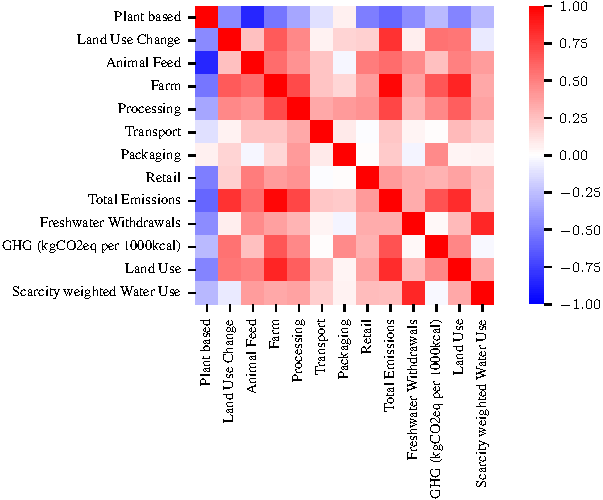
\includegraphics[width=0.65\textwidth]{figures/heat-map.pdf}
  \caption{Correlation of a subset of features depicted in a heatmap. Plant-based products are  anti-correlated ($\rho \in [-1.0, -0.5]$) with every other feature, in particular \textit{Total Emissions}, with the  exception of \textit{Transport} and \textit{Packaging}.}
  \label{fig:corr}
\end{figure}
The code to the data preprocessing and analysis can be found at: \par
\centerline{\url{https://github.com/hannma/data-literacy-project.git}}

\subsection*{Hypothesis Testing}
In order  to decide as to whether the data supports our hypothesis, we will run a T-test, which tests, if the two distributions have equal means (Null-hypothesis).  Since the samples are neither of same size, nor of same variance and are assumed to be independent, we opt for the independent unequal variance T-Test, also known as \textit{Welch's Test} \cite{Welch1947}. 



The test-statistic is computed as follows:
\begin{equation}\label{eq:t-test}
  t = \frac{\bar{X}-\bar{Y}}{\sqrt{\sigma^2_{X}+\sigma^2_{Y}}}
\end{equation}
where $\bar{X}$ and  $\bar{Y}$ are the sample mean with respective standard deviations $\sigma_{X}$ and $\sigma_{Y}$ and we will set the significance level to $\alpha = 0.01$.

\subsubsection*{Do plant- and non-plant-based food products significantly differ with respect to their total emissions?}


 We will consider \textit{plant-based} and \textit{not plant-based} with respect to  the two features \textit{Total emissions} and \textit{GHG (kgCO2eq per 1000kcal)} respectively.
\paragraph*{Kernel density estimation to check for distribution family} Since \textit{Welch's Test} assumes implicitly Gaussian-distributed data, we have to ensure that our assumption of Gaussian distributed data is reasonable.  We therefore generate a histogram and estimate the kernel density with the Python package Seaborn \cite{Seaborn}. Plant-based and not-plant-based food categories are depicted with respect to their total emissions in \Cref{fig:emissions}.

\begin{figure}[h]
  \centering
  \begin{subfigure}[b]{0.49\textwidth}
    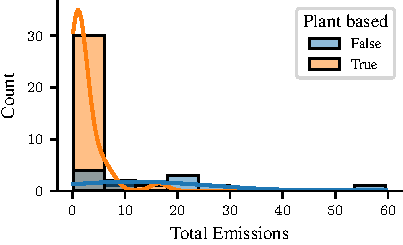
\includegraphics[width=\textwidth]{figures/emissions.pdf}
    \caption{Raw data.}
    \label{fig:emissions}
  \end{subfigure}%
  \hfill
  \begin{subfigure}[b]{0.49\textwidth}
    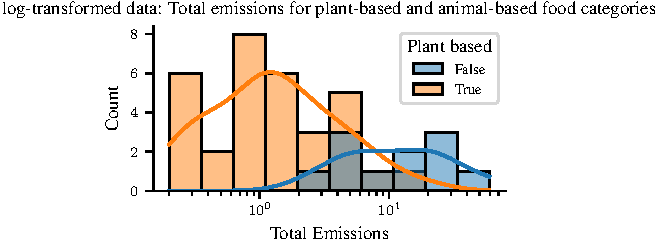
\includegraphics[width=\textwidth]{figures/emissions-log.pdf}
    \caption{Log-transformed data.}
    \label{fig:emissions-log}
  \end{subfigure}
  \caption{Total emissions for plant-based and animal-based food categories.}
  \label{fig:emissions-combined}
\end{figure}

Analyzing \Cref{fig:emissions}, two things can be concluded: First, our hypothesis, that the plant-based and animal-based food products have two different underlying distributions can be confirmed. Second, the distribution over total emissions of plant-based products clearly does not follow a Gaussian distribution. 

\paragraph*{Data transformation}
We apply the logarithm with basis 10 to the data, which is non-negative. Applying the logarithm, we obtain the kernel density estimation depicted in \Cref{fig:emissions-log}.
The transformed data now seem to follow a  Gaussian distribution and we therefore apply the Welch's Test.

\subsubsection*{Accounting  for Nutritional Value: Do plant- and non-plant-based food products significantly differ with respect to their GHG per 1000kcal?}

Since it is very important that everybody has access to diets that meet all the nutritional requirements, we will now consider \textit{plant-based} and \textit{not plant-based} with respect to their nutritional value (feature \textit{GHG in kgCO2eq per 1000kcal}).

\begin{figure}[h]
  \centering
  \begin{subfigure}[b]{0.49\textwidth}
    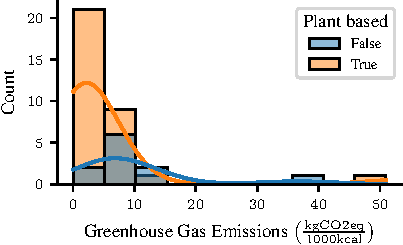
\includegraphics[width=\textwidth]{figures/ghg.pdf}
    \caption{Raw data.}
    \label{fig:ghg}
  \end{subfigure}%
  \hfill
  \begin{subfigure}[b]{0.49\textwidth}
    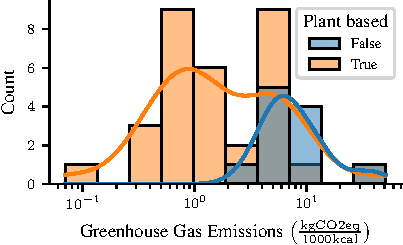
\includegraphics[width=\textwidth]{figures/ghg-log.pdf}
    \caption{Log-transformed data.}
    \label{fig:ghg-log}
  \end{subfigure}
  \caption{GHG-Emissions (kgCO2eq per 1000kcal) for plant-based and animal-based food categories.}
  \label{fig:ghg-combined}
\end{figure}

% \begin{figure}[h]
%     \centering
%     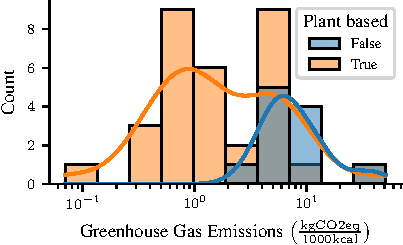
\includegraphics[width=0.5\textwidth]{figures/ghg-log.pdf}
%     \caption{Log-transformed data: GHG-Emissions (kgCO2eq per 1000kcal) for plant-based and animal-based food categories}
%     \label{fig:ghg-log}
% \end{figure}



\subsection{Comparing Example Diets}
We now take an even more granular view at the nutritional value of (non) plant-based diets by considering two typical diets with respect to recommended macro-nutrient make-up (carbohydrates, fat, protein).

\paragraph*{Diet calories and nutrients composition}
The consumer of these diets is an average woman, whose daily calories intake is around $2000$kcal \cite{NHS}. The division amongst macro-nutrients was taken from \citet{Healthline} and is depicted in  \Cref{tbl:composition}.

\begin{table}[h]
  \caption{Average woman's daily nutrients intake}
  \label{tbl:composition}
  \centering
  \begin{tabular}{lll}
    \toprule
    Macronutrient     & Suggested percentage of calories   & Daily grams for the average woman  \\
    \midrule
    Carbohydrates & $45\%-65\%$ &  225g-325g  \\
    Fats    & $20\%-35\% $  & 45g-78g \\
    Proteins & $10\%-35\%$ & 50g-175g \\
    \bottomrule
  \end{tabular}
\end{table}

\paragraph*{What the example diets contain}
The following diets are described by the amount of food category consumed in a day in order to reach the suggested intake of nutrients, thus not considering specific recipes or meals, nore guidelines about correct division in ingredients categories. Note that food categories are named the same as they are named in the dataset used in this research, while nutritional facts of the different foods can easily be found on various famous health websites. The crafted diets are shown in \Cref{tbl:plantdiet} and \Cref{tbl:omnidiet}.

\begin{table}[h]
\parbox{.45\linewidth}{
  \caption{Exemplatory Plant-based  Diet}
\centering
\begin{tabular}{c c}
\toprule
Food Category & Grams\\
\midrule
Wheat \& Rye (Bread) & 400\\
Tofu & 300\\
Bananas & 300\\
Peas & 200\\
Nuts & 50\\
Soymilk & 150\\
\bottomrule
\end{tabular}
\label{tbl:plantdiet}
}
\hfill
\parbox{.45\linewidth}{
  \caption{Exemplatory Omnivor  Diet}
\centering
\begin{tabular}{c c}
\toprule
Food Category & Grams\\
\midrule
Wheat \& Rye (Bread) & 400\\
Pig Meat & 200\\
Bananas & 300\\
Cheese & 150\\
\bottomrule
\end{tabular}
\label{tbl:omnidiet}
}
\end{table}

\paragraph*{Emissions calculation} The total emissions of a daily diet has been computed by the sum of the single contributions of every food category in kgCO2eq per kg, each calculated in proportion of the amount consumed in the diet as in \Cref{eq:diet}.

\begin{equation}\label{eq:diet}
  \textrm{Emissions}_{\textrm{food}} = \frac{\textrm{Total Emissions of the food category} \cdot \textrm{Grams contained in the diet}}{1000g}
\end{equation}

\section{Results}
\begin{table}[h]
  \caption{Results of  Welch's Hypothesis Test}
  \label{tbl:results-test}
  \centering
  \begin{tabular}{lll}
    \toprule
    %\multicolumn{1}{c}{}&\multicolumn{2}{c}{Plant-based} &%\multicolumn{2}{c}{Animal-based}                   \\
    %\cmidrule(r){2-5}
    Feature     & Test-Statistic   & p-value  \\
    \midrule
    Total Emissions &$\approx 6.49$  & $ 2.2\cdot10^{-6}  $  \\
    GHG (kgCO2eq per 1000kcal)    & $\approx 5.03 $  & $ 1.4\cdot10^{-5}$    \\
    \bottomrule
  \end{tabular}
\end{table}

\begin{table}[h]
  \caption{Results of diet emissions calculation}
  \label{tbl:results-diets}
  \centering
  \begin{tabular}{ll}
    \toprule
    %\multicolumn{1}{c}{}&\multicolumn{2}{c}{Plant-based} &%\multicolumn{2}{c}{Animal-based}                   \\
    %\cmidrule(r){2-5}
    Diet    & Emissions in kgCO2eq  \\
    \midrule
    Plant-based & $2.02$\\
    Omnivor    &  $5.42$\\
    \bottomrule
  \end{tabular}
\end{table}

Based on statistical analysis we found that not only total emissions but also GHG emissions when accounting for nutritional value (in kgCO2eq per 1000kcal) have a p-value of  $p= 2.2\cdot10^{-6} $  and $p= 1.4\cdot10^{-5}$  when conducting the unequal variance test with $\alpha = 0.01$ (see \Cref{tbl:results-test}). With regards to the diet examples comparison, as seen in \Cref{tbl:results-diets} the plant-based diet emits $2.02$ kgCO2eq while the omnivor one emits $5.42$ kgCO2eq, i.e. $268\%$ of the first one.

\section{Conclusion}
\label{conclusion}
Our results demonstrate a significant difference between plant- and animal-based products, not only with respect to their total emissions but also when accounting for nutritional value. Thus, plant-based diets not only seem to satisfy nutritional requirements \cite{WHO2021} but importantly, also would contribute significantly to solving climate change when consumed by many. Importantly, eating more plant-based is a clear rule that would help individuals willing to contribute to solving climate change make more informed decisions in their daily life. 

\section{Limitations and Outlook}
\label{limitations}
Limitations start in the data collection process and stretch into the analysis part, both of which strongly influence the study's plausibility and impact. Some critical points will be briefly discussed for both aspects, followed by  a brief outlook on future work that could be done.

\paragraph*{Limitations in the data}
A wide variety of fruits  are  available year-round in Western grocery stores  irrespective as to whether  they are in season or are native to the Northern hemisphere. 
Seasonality is not considered in the data collection process but clearly affects both energy for cooling potentially transport and hence total emissions.  
A potential solution to control for this confounding variable seasonality might be, to first introduce this information in the data-collection process and second, to condition on this variable in the analysis part.

Furthermore, it is arguably up for discussion as to how different greenhouse gases are weighted  when calculating the ``carbon dioxide-equivalents (CO$_{2}$eq)'' as described in  \Cref{data}. For instance, methane is a much shorter-loved but more powerful greenhouse gas than CO$_{2}$.




\paragraph*{Limitations in the analysis}
First of all, the assumption of Gaussian-distributed data may be criticized and the following T-Test, which implicitly assumes Gaussian distributed data.
In particular, the data of plant-based food depicted in \Cref{fig:ghg-log} seems to follow a bimodal distribution as opposed to a Gaussian distribution.
Second, a more granular analysis regarding the variance within each food-group would be interesting. This could elude to the differences of producers regarding greenhouse gas emissions and may therefore provide the opportunity to further minimize emissions during the food-production process by optimizing towards the lowest-emitting producers. 

\paragraph*{Outlook and future work}

Having data by country available would be  very interesting and useful to identify areas, which present a lot of room for improvement in terms of emissions. Based on emissions by country, a more granular distinction regarding  as to how much of a country's  emissions go towards exporting and how many greenhouse gases are accounted for  imported  goods, would be very insightful as well. Such an analysis would give further insights with respect to detecting more and less efficient countries and would hence give room for further minimizing emissions in the less-efficient countries and hence would minimize the global emissions.

While there are some concerns, that vegan diets (i.e, plant-based diets that exclude all forms of animal products in their entirety) are not sufficient with respect to providing recommended micronutrient levels (e.g., vitamin B12, zinc, iron, etc.), they generally meet protein intake recommendations \cite{WHO2021}. In particular, the food-groups  used in the dataset used in this study represent   about 90\% of global calorie and protein-intake. Nonetheless, individuals who consume a vegan diet should remain aware regarding potential micronutrient insufficiencies and further research on that end would certainly be insightful.

  
{\small
\bibliographystyle{unsrtnat}
\bibliography{../literature/references.bib}
}
\end{document}
